\section{Frontend}
Das Frontend für den Feasibility Check basiert auf der bereits implementierten Web\-oberfläche des \gls{REALIS}-Systems und wurde so erweitert, dass die Funktionalität des Feasibility Checks nahtlos in die bestehende Anwendung für den \glsentrylong{QM} integriert wird. Dadurch entfällt die Notwendigkeit, das Projekt an das \gls{RPT}-Labor zu übergeben, um den Check durchzuführen. Das neue, automatisierte System ermöglicht es dem \gls{QM}, die Machbarkeit der angelegten Tests eigenständig und ohne externe Laborunterstützung zu überprüfen.

Zuvor muss der \gls{QM} ein neues \gls{REALIS}-Projekt für ein zu qualifizierendes Produkt anlegen. Dieses Projekt kann mehrere unterschiedliche Tests enthalten, wobei der Nutzer durch vorgefertigte Templates unterstützt wird, die gängige Testkonfigurationen und zugehörige Daten bereitstellen. Nach Abschluss der Projekterstellung gelangt der Benutzer auf die Hauptoberfläche, wie in Abbildung~\ref{fig:whole-page} dargestellt.

\begin{figure}[!htbp] 
    \centering 
    \makebox[\textwidth]{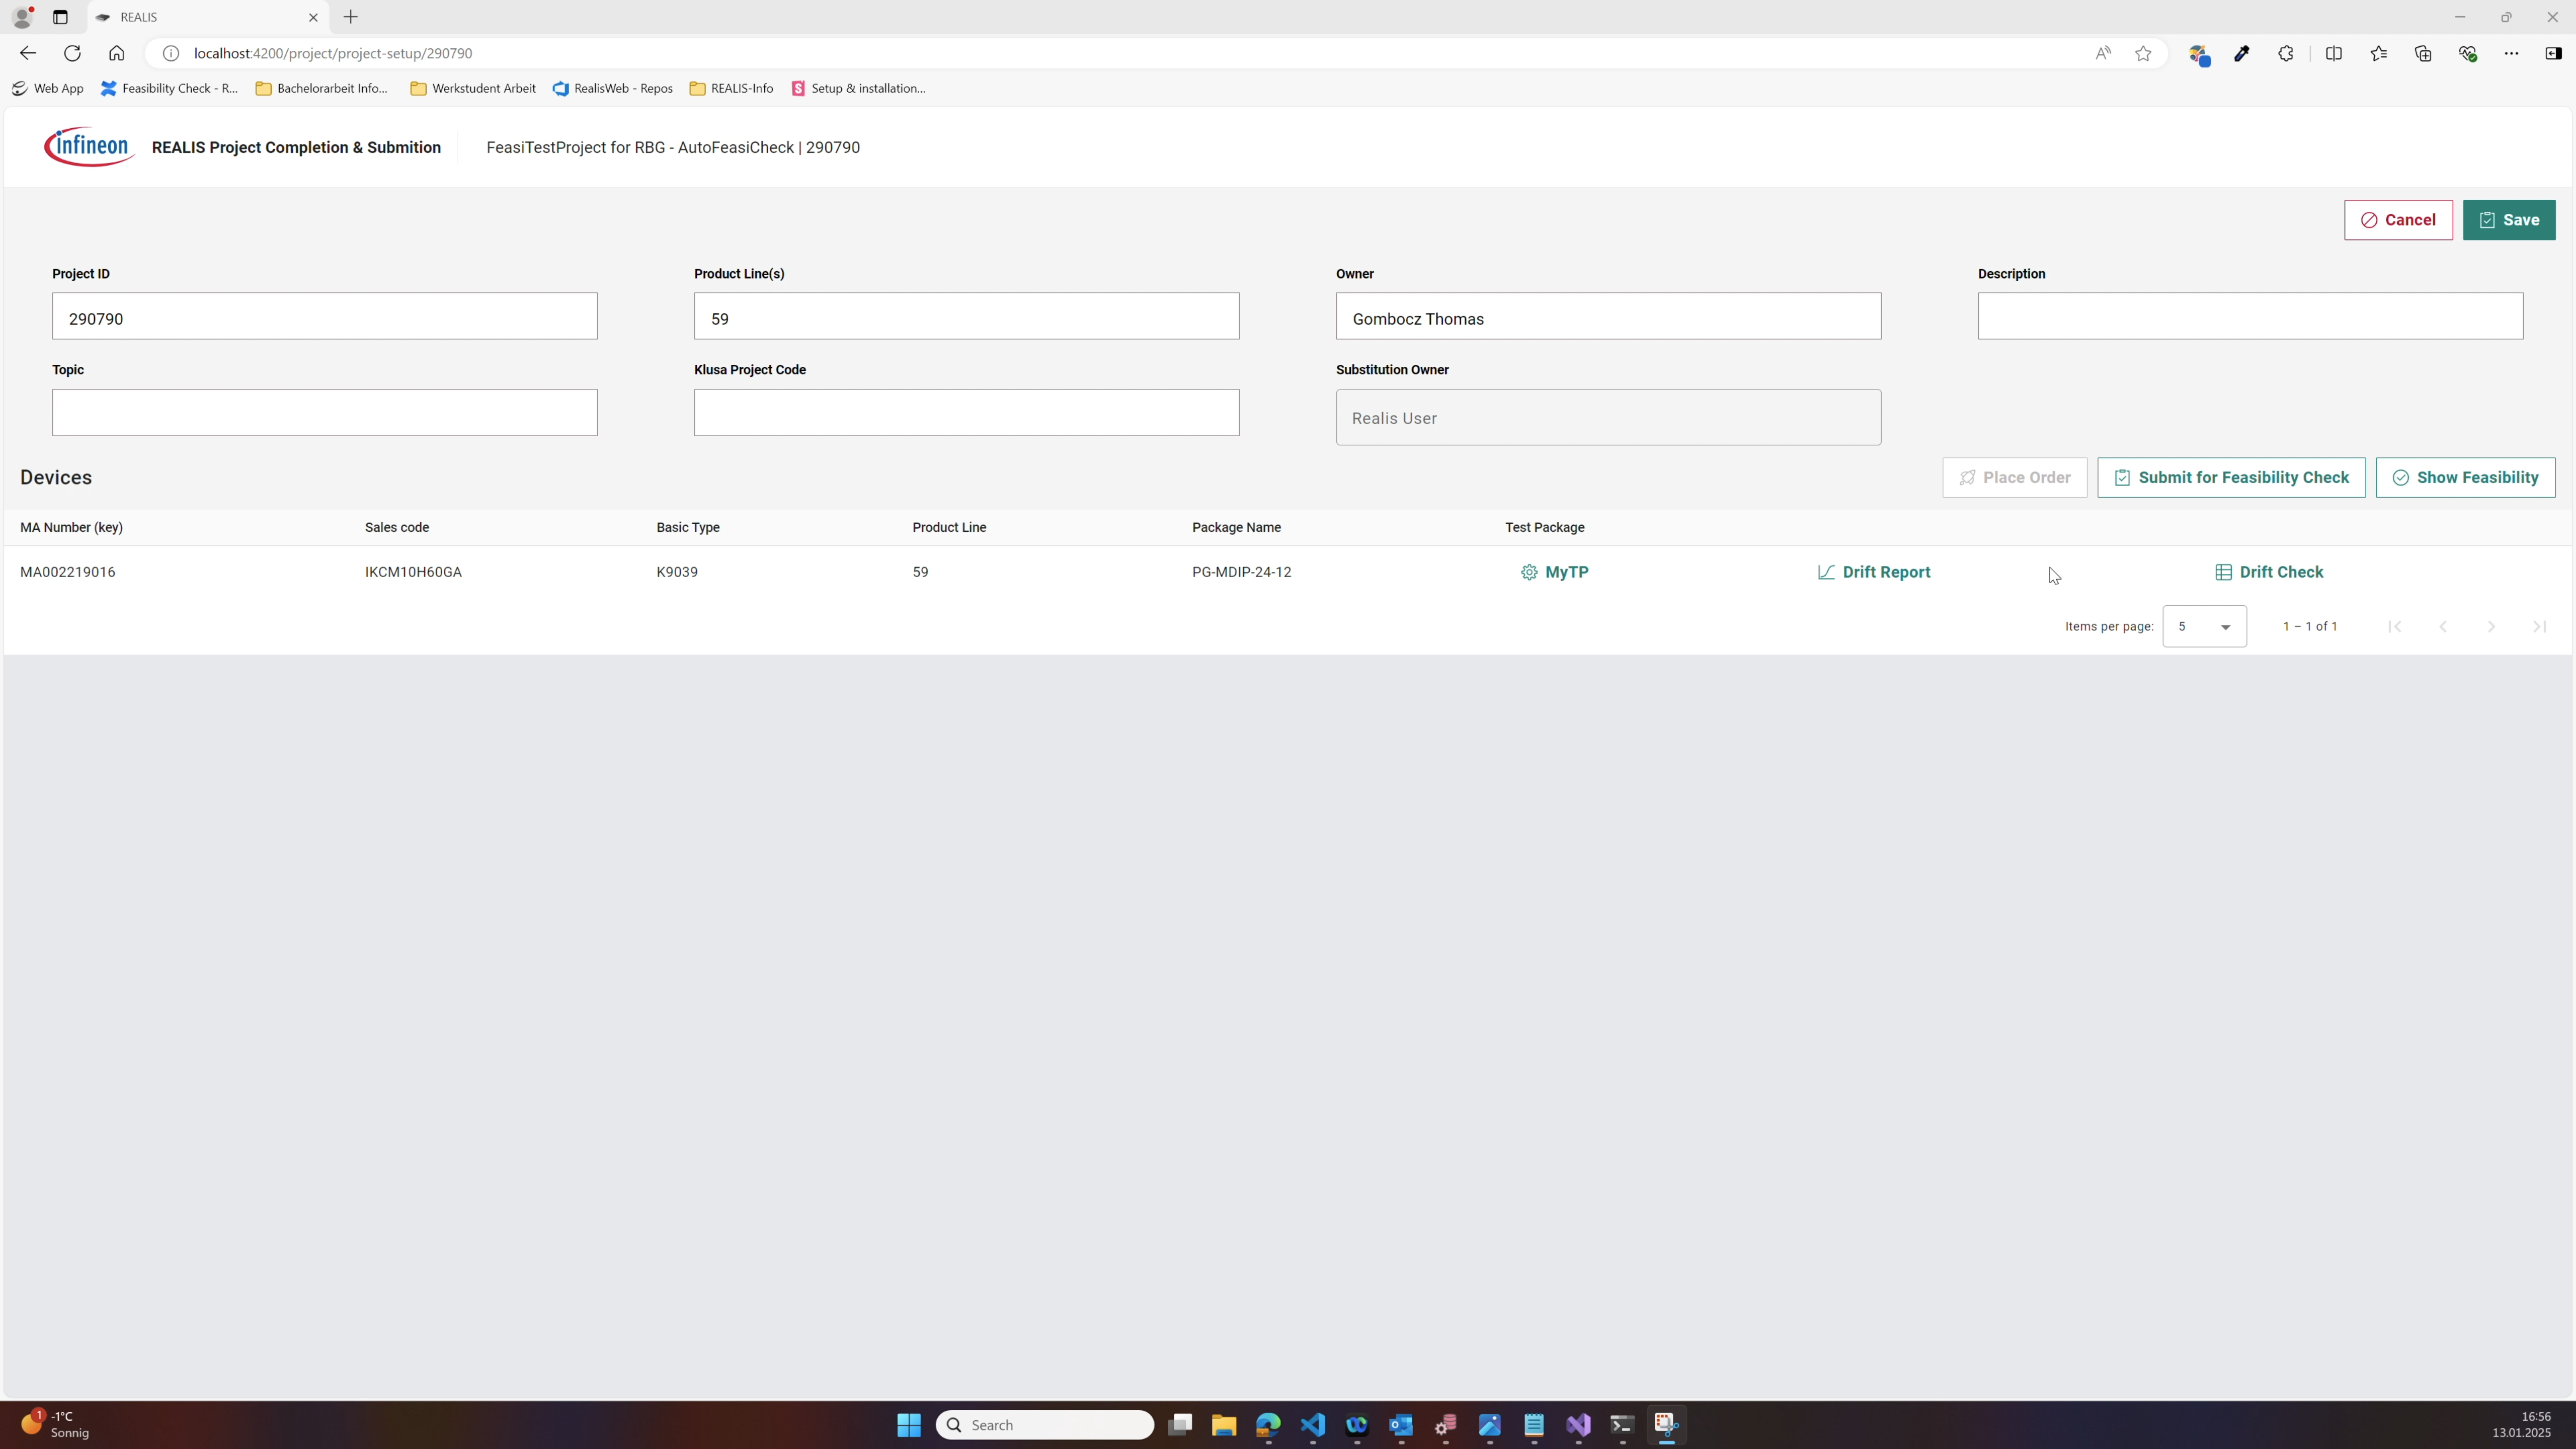
\includegraphics[width=0.85\paperwidth]{bilder/frontend/whole-page.png}} 
    \caption{Weboberfläche für den Quality Manager (QM) – Einstiegspunkt für den Feasibility Check} 
    \label{fig:whole-page} 
\end{figure}

Auf dieser Oberfläche kann der Feasibility Check für die definierten (Stress-)Tests durchgeführt werden. Hierfür befindet sich ein grün umrandeter Button mit der Beschriftung ''Submit for Feasibility Check'' auf der rechten Seite der Website (siehe Abb. \ref{fig:whole-page}). Wird dieser Button betätigt, öffnet sich ein Popup-Fenster (Modal-Page), das dem Nutzer eine Übersicht der angelegten Tests in tabellarischer Form präsentiert. Diese Tabelle enthält die wichtigsten Informationen, wie den Teststatus und die eindeutige Test-ID (siehe Abbildung \ref{fig:submit-page}).

\subsection{Modal-Page für die Initiierung des Feasibility Checks}

Innerhalb der Modal-Page kann der Benutzer mittels CheckBoxen die einzelnen Tests auswählen, die den Feasibility Check durchlaufen sollen. Alternativ besteht die Möglichkeit, alle Tests simultan auszuwählen, indem die oberste CheckBox in der Spaltenüberschriftenleiste aktiviert wird (siehe Mauszeigerposition in Abbildung \ref{fig:submit-page}).

\begin{figure}[!htbp] 
    \centering 
    \makebox[\textwidth]{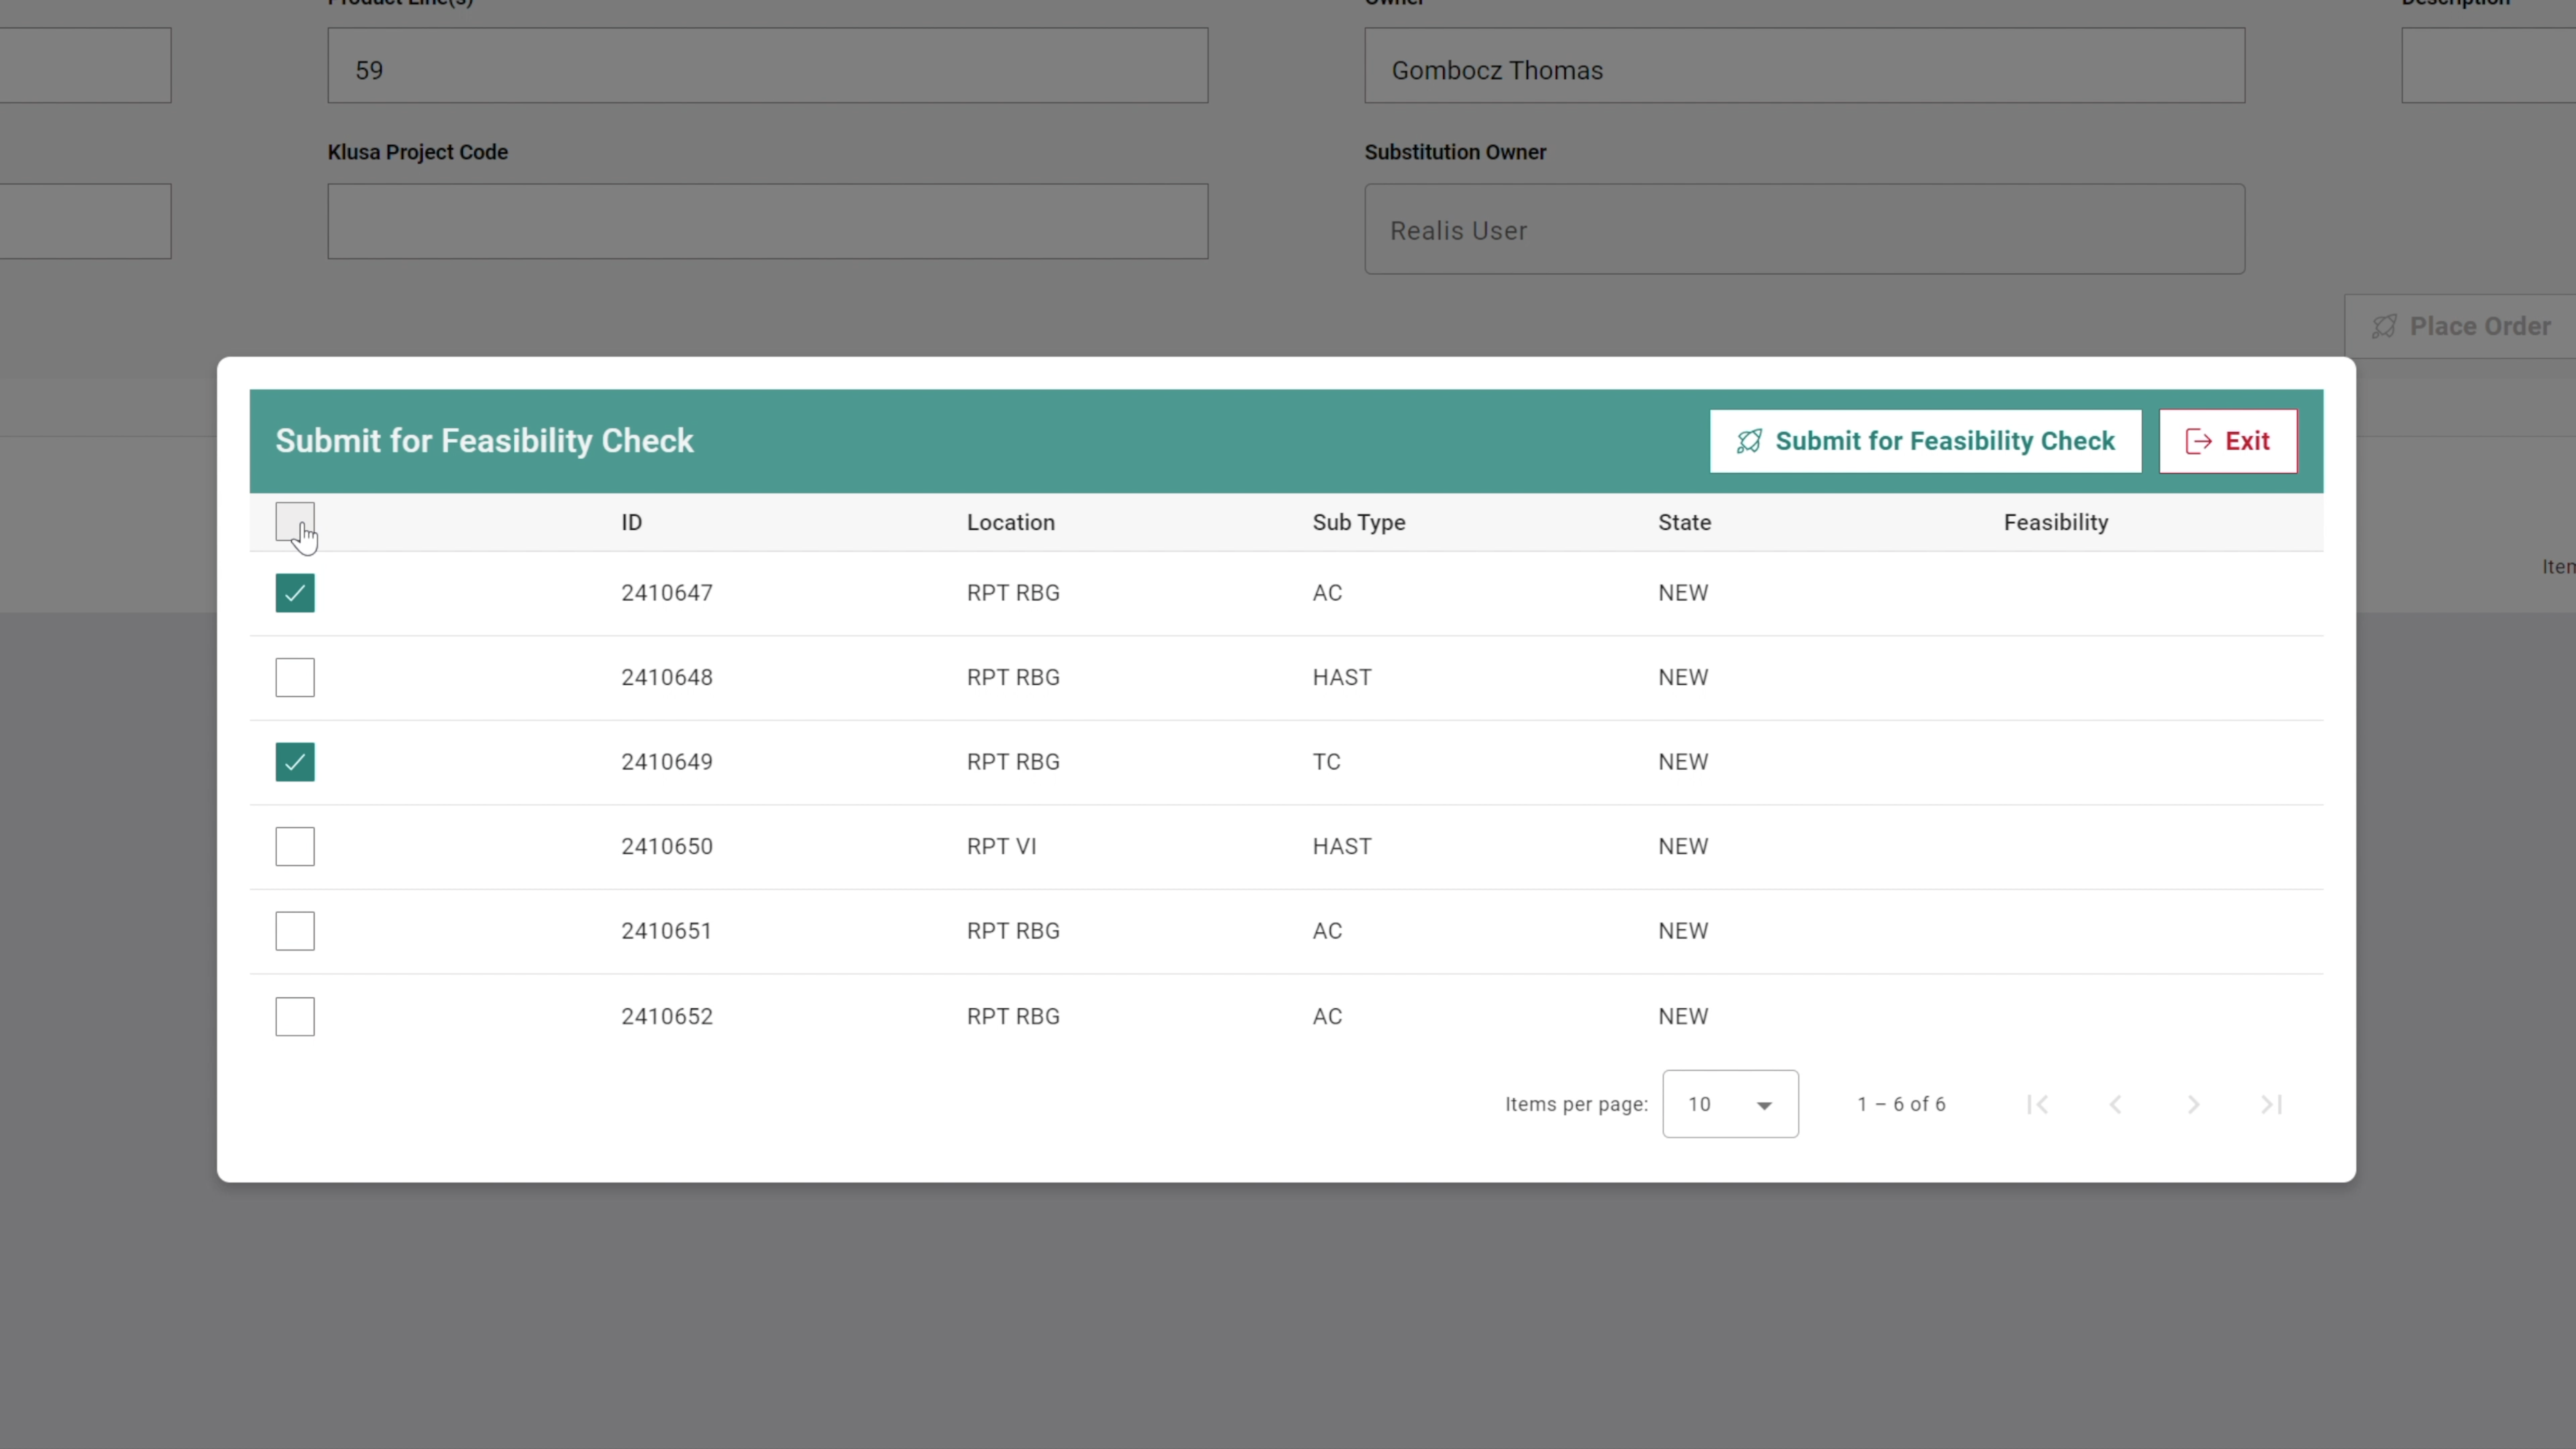
\includegraphics[width=0.85\paperwidth]{bilder/frontend/feasibility-modal-page.png}} 
    \caption{Modal-Page ''Submit for Feasibility Check'' – Modal-Page zur Initiierung des Feasibility Checks} 
    \label{fig:submit-page} 
\end{figure}

Nachdem der Benutzer die gewünschten Tests selektiert hat, klickt er auf den ''Submit for Feasibility Check''-Button, der oben rechts im Popup, links neben dem ''Exit''-Button, positioniert ist. Mit diesem Klick wird für jeden ausgewählten Test ein asynchroner HTTP-Call an die Backend-Logik initiiert. Über die REST-API wird dabei die Helfer-Methode aufgerufen, wobei die jeweilige Test-ID als Parameter übermittelt wird.

Die asynchronen HTTP-Calls erlauben es dem Benutzer, während der Durchführung der Überprüfungen weiterhin mit der Oberfläche zu interagieren.\todo{hier könnte wieder auf Anforderungen verwiesen werden} So kann das Popup-Fenster ohne Unterbrechung des laufenden Feasibility Checks geschlossen oder für andere Aktionen genutzt werden. In der „Feasibility“-Spalte rechts wird der Fortschritt des Checks durch rotierende Ladekreise visualisiert (siehe Abbildung \ref{fig:loading-with-results}). Je nach Feasibility-Konfiguration und Komplexität des Tests dauert die Überprüfung etwa zwei bis 15 Sekunden, bis die ersten Ergebnisse vorliegen.\todo{hier auch}

\begin{figure}[!htbp] 
    \centering 
    \makebox[\textwidth]{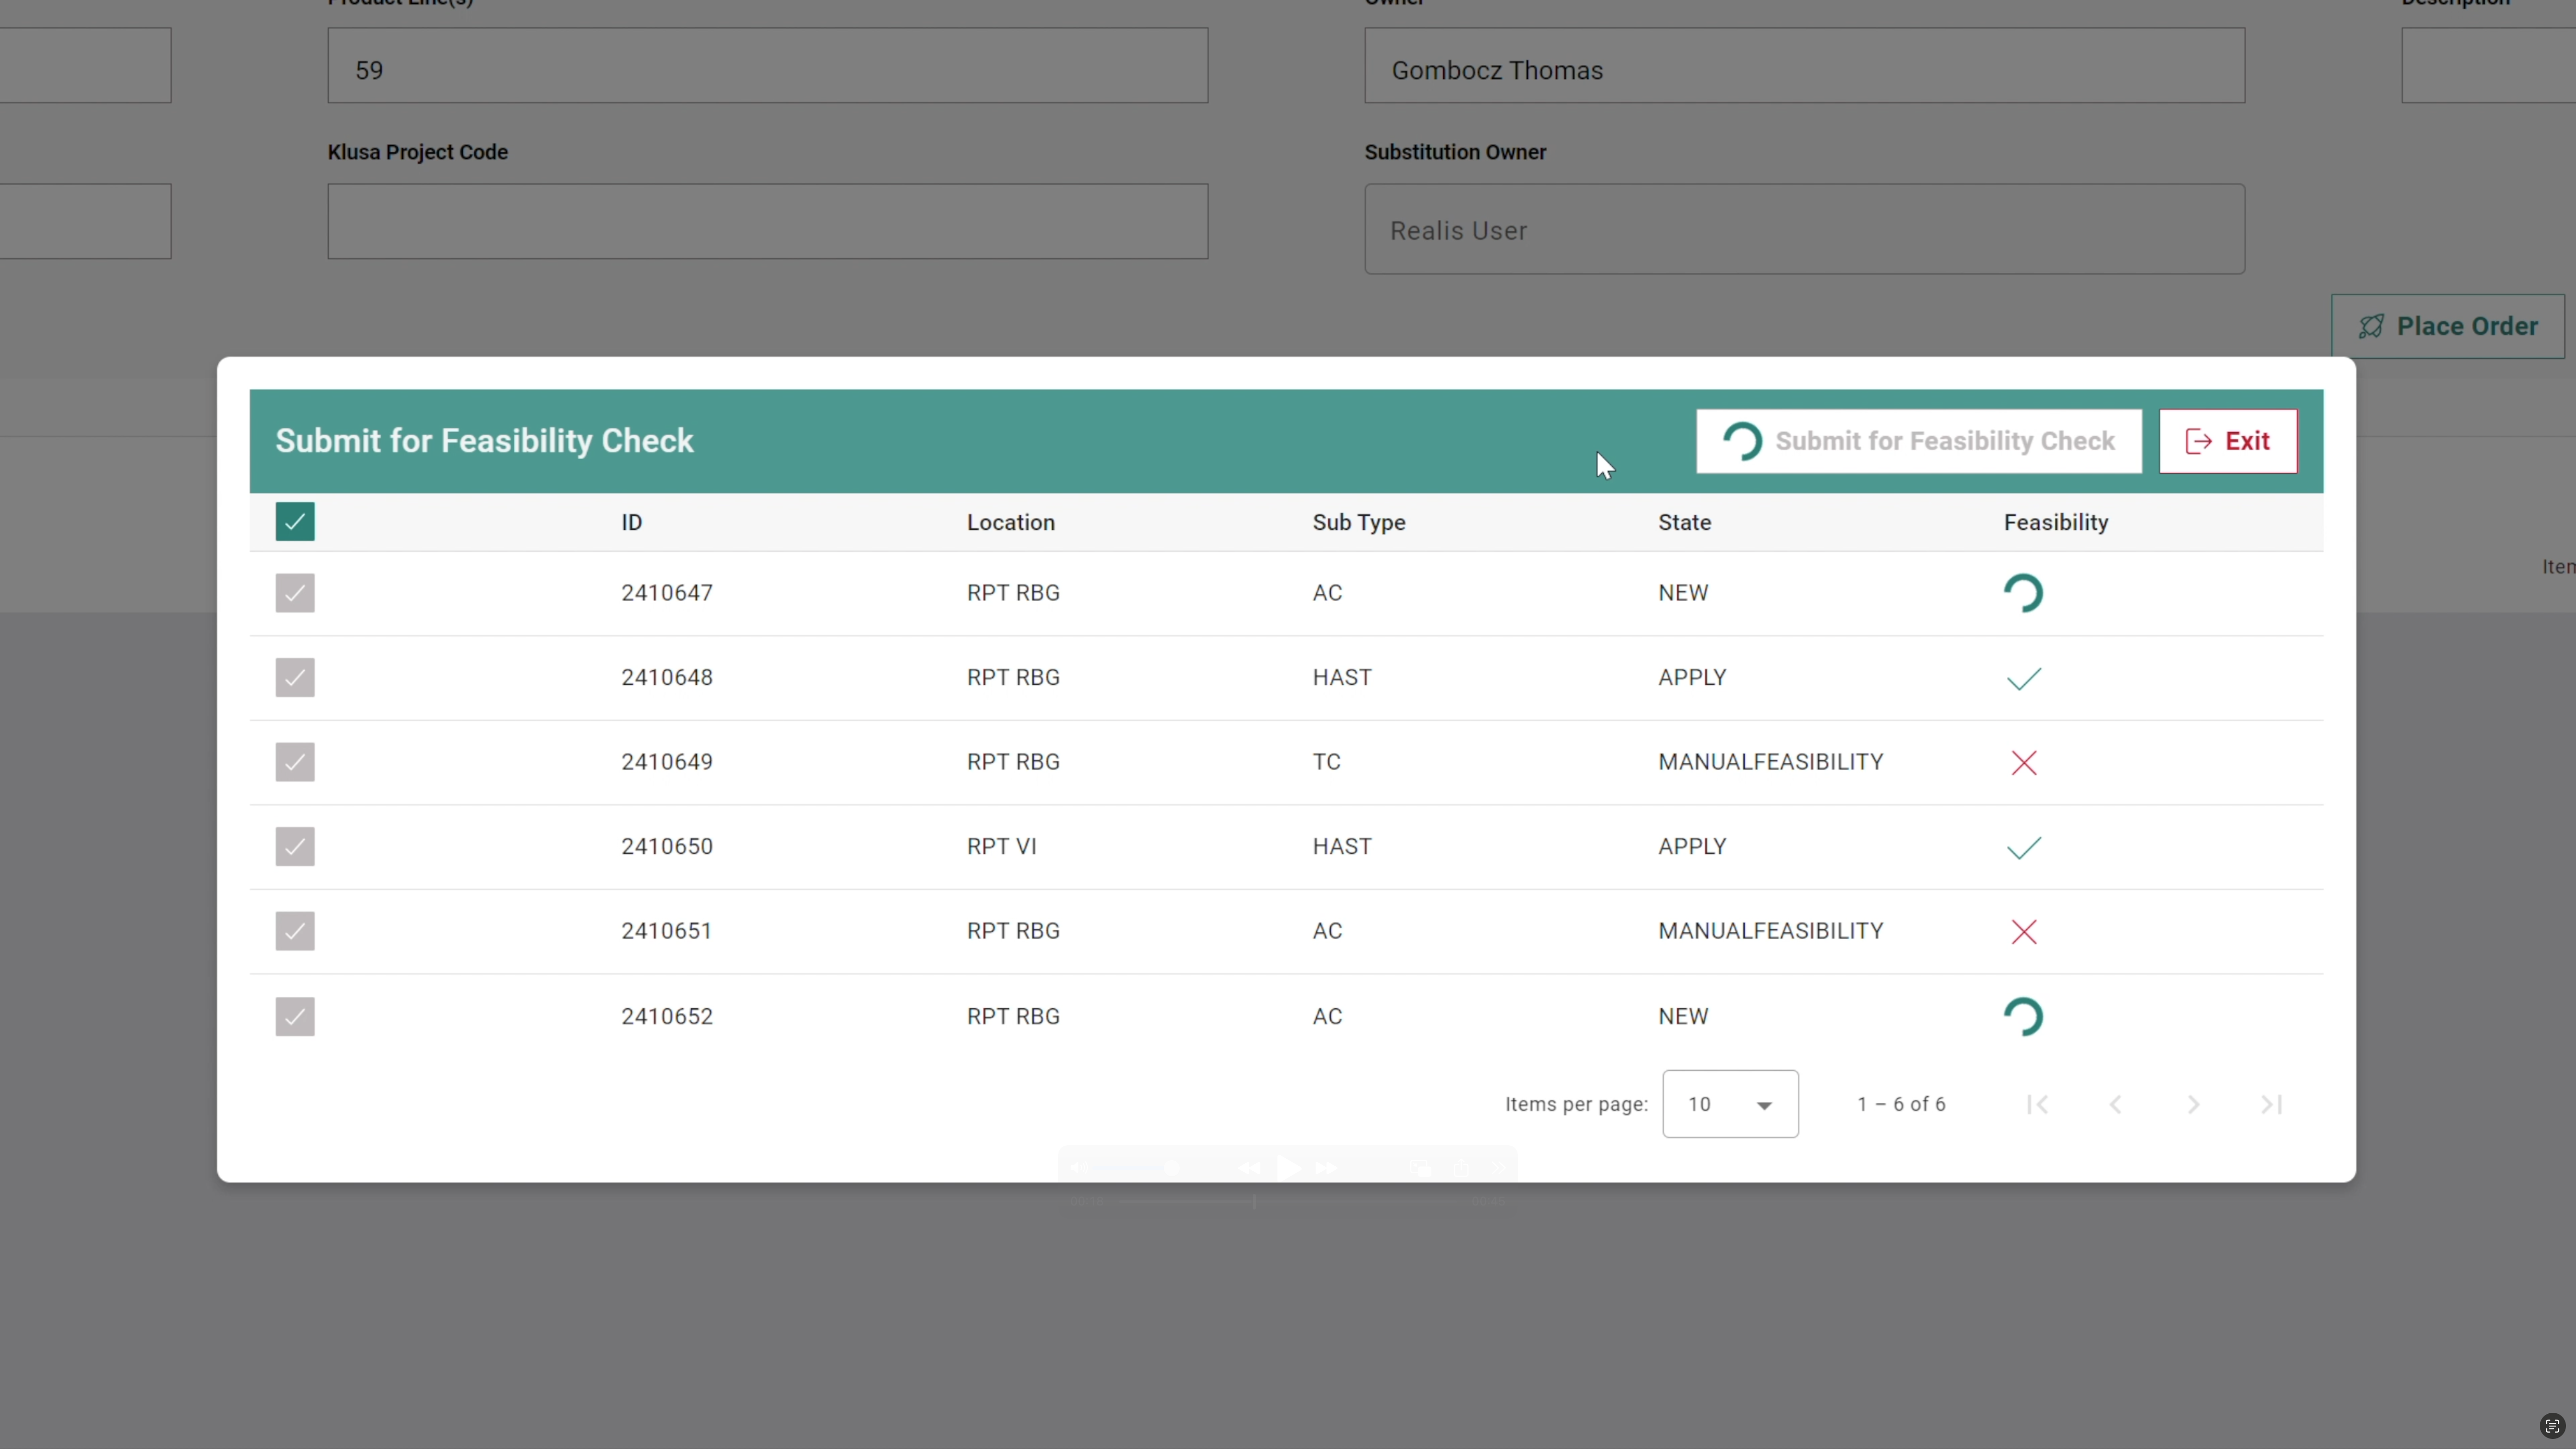
\includegraphics[width=0.85\paperwidth]{bilder/frontend/loading-with-results.png}} 
    \caption{Modal-Page ''Submit for Feasibility Check'' – Ladevorgang und erste Ergebnisse} 
    \label{fig:loading-with-results} 
\end{figure}

Sobald einzelne Überprüfungen abgeschlossen sind, wird der entsprechende Ladekreis durch ein Status-Icon ersetzt und der Teststatus in der Übersicht aktualisiert (siehe Abb. \ref{fig:loading-with-results}). Ein grüner Haken sowie der Status ''APPLY'' signalisieren, dass der Feasibility Check erfolgreich abgeschlossen wurde. Erscheint hingegen ein rotes Kreuz und der Status ''MANUALFEASIBILITY'', so weist dies darauf hin, dass ein oder mehrere Kriterien nicht erfüllt wurden oder der Test in der Konfiguration noch nicht für eine automatisierte Überprüfung freigeschaltet ist. In beiden Fällen muss der Test manuell von einem Mitarbeiter überprüft werden.

Tritt ein Fehler im Algorithmus auf, erscheint ein rotes Dreieck mit Ausrufezeichen. In diesem Fall bleibt der Test-Status unverändert oder wird auf ''FEASIBILITY\-REQUEST'' gesetzt, je nachdem wann und welcher Fehler auftritt (dieser Fall ist in der Abbildung \ref{fig:loading-with-results} nicht dargestellt).


\subsection{Modal-Page für detaillierte Ergebnisse des Feasibility Checks}

Nach Abschluss der Feasibility Checks für einzelne Tests kann der Benutzer über einen separat positionierten, grün umrandeten ''Show Feasibility''-Button in der Start\-oberfläche (siehe Abbildung~\ref{fig:whole-page}) detaillierte Ergebnisse einsehen. Beim Betätigen dieses Buttons öffnet sich eine zweite Modal-Page, die in Abbildung~\ref{fig:result-details} dargestellt ist.

\begin{figure}[!htbp] 
    \centering 
    \makebox[\textwidth]{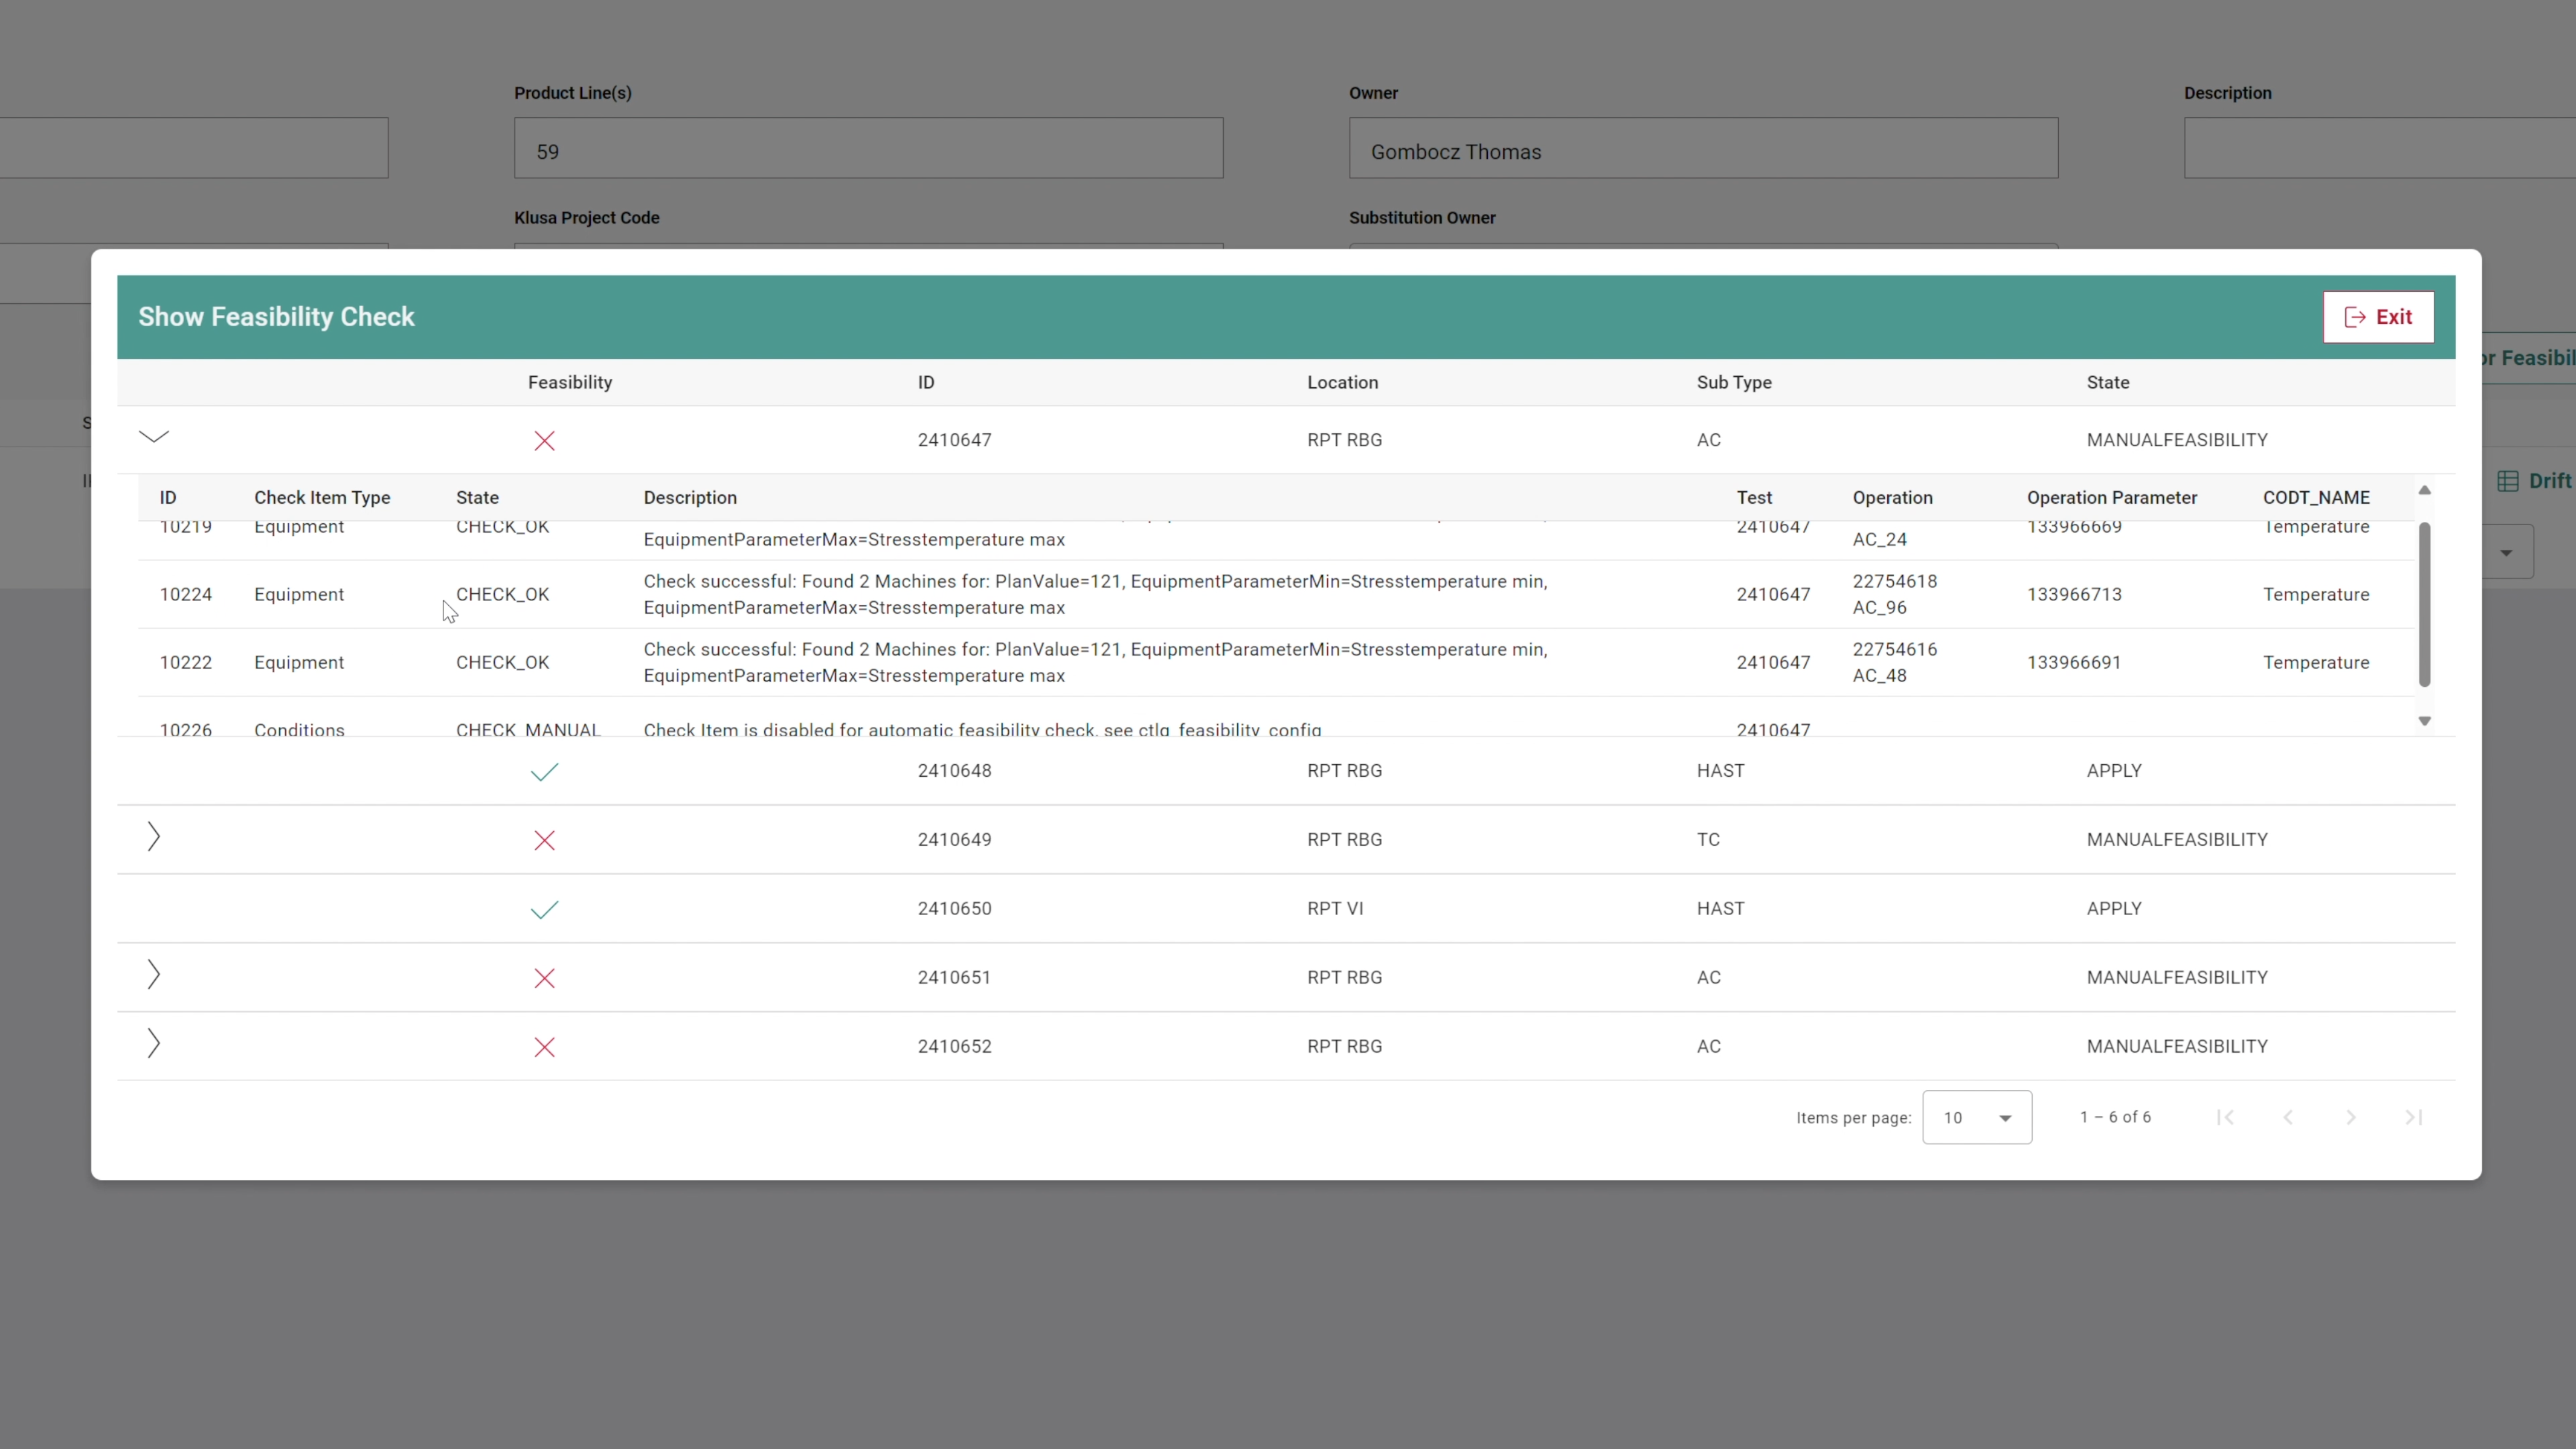
\includegraphics[width=0.85\paperwidth]{bilder/frontend/result-details.png}} 
    \caption{Modal-Page ''Show Feasibility Check'' – Detaillierte Ergebnisse des Feasibility Checks} 
    \label{fig:result-details} 
\end{figure}

Diese Seite zeigt in tabellarischer Form alle Tests zusammen mit den zugehörigen Ergebnissen. Über ein Aufklappmechanismus können einzelne Testzeilen erweitert werden, sodass detaillierte Informationen – die gespeicherten \texttt{feasibility\_check\_item\_results} – eingesehen werden können. Bei Tests, die ausschließlich den Status \texttt{CHECK\_OFF} aufweisen, können keine zusätzlichen Details angezeigt, da in diesen Fällen in der Regel keine Feasibility-Resultate abgespeichert werden.

Innerhalb der Detailansicht wird neben dem Typ des CheckItems (Condition oder Equipment Check) auch der jeweilige (End-)Status, wie er in der Backend-Logik definiert ist, dargestellt (siehe Tabelle \ref{tab:feasibility-states}). Ergänzend dazu wird das Nutzer-Feedback, welches in Kapitel \ref{Subsec:user-feedback} beschrieben wurde, angzeigt und liefert weiterführende Informationen zu dem jeweiligen Check. Falls vorhanden, werden auch der zugehörige Operationstyp sowie die Parameter-ID angezeigt.

Diese detaillierte Darstellung unterstützt den Benutzer dabei, die Ergebnisse des Feasibility Checks nachvollziehen zu können und gegebenenfalls notwendige Anpassungen an den geplanten Tests, den zugehörigen Parameterwerten oder den Einträgen in der Konfigurationstabelle vorzunehmen.

Insgesamt trägt das integrierte Frontend-Design wesentlich dazu bei, die Benutzerfreundlichkeit und Transparenz des Feasibility Checks zu erhöhen. Durch die intuitive Bedienung und die asynchrone Verarbeitung der Prüfprozesse wird es dem \gls{QM} ermöglicht, effizient und selbstständig die Machbarkeit der Tests zu evaluieren und bei Bedarf zeitnah entsprechende Maßnahmen zu ergreifen.


